Dado un conjunto de puntos, encuentre el par más cercano (con cualquier métrica). Por supuesto, esto puede resolverse en tiempo O($N^2$) considerando todos los pares, pero un barrido de línea puede reducirlo a O($N\log N$).

Supongamos que hemos procesado los puntos $1$ a $N-1$ (ordenados por $x$) y la distancia más corta que hemos encontrado hasta ahora es $h$. Ahora procesamos el punto $N$ e intentamos encontrar un punto más cercano a él que $h$. Mantenemos un conjunto de todos los puntos ya procesados cuyas coordenadas $X$ están dentro de $h$ del punto $N$, como se muestra en el rectángulo gris claro. A medida que se procesa cada punto, se agrega al conjunto, y cuando pasamos al siguiente punto o cuando se disminuye $h$, los puntos se eliminan del conjunto. El conjunto está ordenado por la coordenada $y$. Un árbol binario balanceado es adecuado para esto y representa el factor $\log N$.

% TODO: \usepackage{graphicx} required
\begin{figure}[h!]
	\centering
	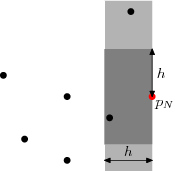
\includegraphics[width=0.2\linewidth]{img/closest}
	\label{fig:closest}
\end{figure}

Para buscar puntos más cercanos que $h$ al punto $N$, solo necesitamos considerar puntos en el conjunto activo y, además, solo necesitamos considerar puntos cuyas coordenadas y estén en el rango $N_y - h$ a $N_y + h$ (aquellos en el rectángulo gris oscuro) . Este rango se puede extraer del conjunto ordenado en tiempo O($\log N$), pero lo que es más importante, el número de elementos es O($1$) (el máximo exacto dependerá de la métrica utilizada), porque la separación entre dos puntos cualesquiera en el conjunto es al menos $h$. De ello se deduce que la búsqueda de cada punto requiere un tiempo O($\log N$), dando un total de O($N\log N$).